\chapter{Development}
Initially, the algorithm should be able to take an existing non-empty graph as input. This graph can initially be seen as static and therefore HyperBall can perform a complete calculation on it. After HyperBall has completed, the calculated counters can be used as initial counters for the dynamic algorithm. For every insertion and deletion in the dynamic graph, these initial counters are manipulated. If an edge is added, nodes might reach more nodes than before and their counters should be raised. Similarly for deletions, if an edge is deleted, nodes might reach fewer nodes and their counters should be decreased.


\section{Dynamic graphs}

The first thing required for a dynamic graph is the ability to insert new nodes and edges (called entries in this section) to an existing graph. The graph files used by HyperBall are tightly compressed in a byte stream, which makes it an expensive operation to modify the graph at an arbitrary point. This makes it infeasible to insert every additional entry directly into the graph file. Instead, new entries can be stored in some other data structure.

The additional entries could either be stored in a high-level data structure or a byte stream. Keeping them in a high-level data structure will consume a significant amount of storage already at a low number of extra entries. A high-level data structure takes up more memory as each number is always the same size no matter what the value is. For example, the value 3 can be expressed by two bits but a high level integer always take a fixed amount of bits to express this.  Additionally, if each node has a structure containing the neighbors, a significant amount of space will be taken by the pointers to those structures. The compression of the graph is also lost when using a high-level structure.

If a byte stream is used, it is the same problem as the original. Even though this byte stream will be smaller, there will be a point where it is unreasonable to resize the stream and reposition the existing entries at each new entry. Regardless of which method is used, the extra entries and the original graph have to be merged into a new graph at some point. 

\subsection{Merging two graphs with webgraph}

The webgraph framework has a way to create a new graph $G$ by taking the union of two sub graphs $G_1$ and $G_2$. The graph $G$ works by simultaneously reading from the streams of $G_1$ and $G_2$ to produce the nodes and their neighbors. The sub graphs can be unions as well which means that an arbitrary number of graphs can be joined using this method. However, having lots of recursive unions create a large overhead in time  when fetching nodes and edges. \cite{webgraph} 

The framework also supports writing a union-graph to disk as a new graph. Loading this new written graph removes the overhead of several recursive unions. As the graph express some arcs by references to previous arcs, the creation is slow and doesn't leverage any of the calculations already made by the existing graphs. Ignoring the references will make the graphs bigger but it increases the running time of the merge.

The performance difference between unioning graphs and directly merging a graph can be seen in figure \ref{fig:firstIterationUnionVsStored}. Two graphs are used, both originally containing the in-2004 graph. For 50 iterations 1.000 edges are randomly generated and inserted into both graph. One of the graphs only use unions while the other merge the new edges directly into the graph and stores it. The time measured is the time to add the edges and then performing a complete edge scan. This time is saved after each iteration. During the first six iterations, the unioned graph performs faster than the merged. The union scales linearly with the number of unions while the merged graph has constant performance.  

\begin{figure}[h]
\centering
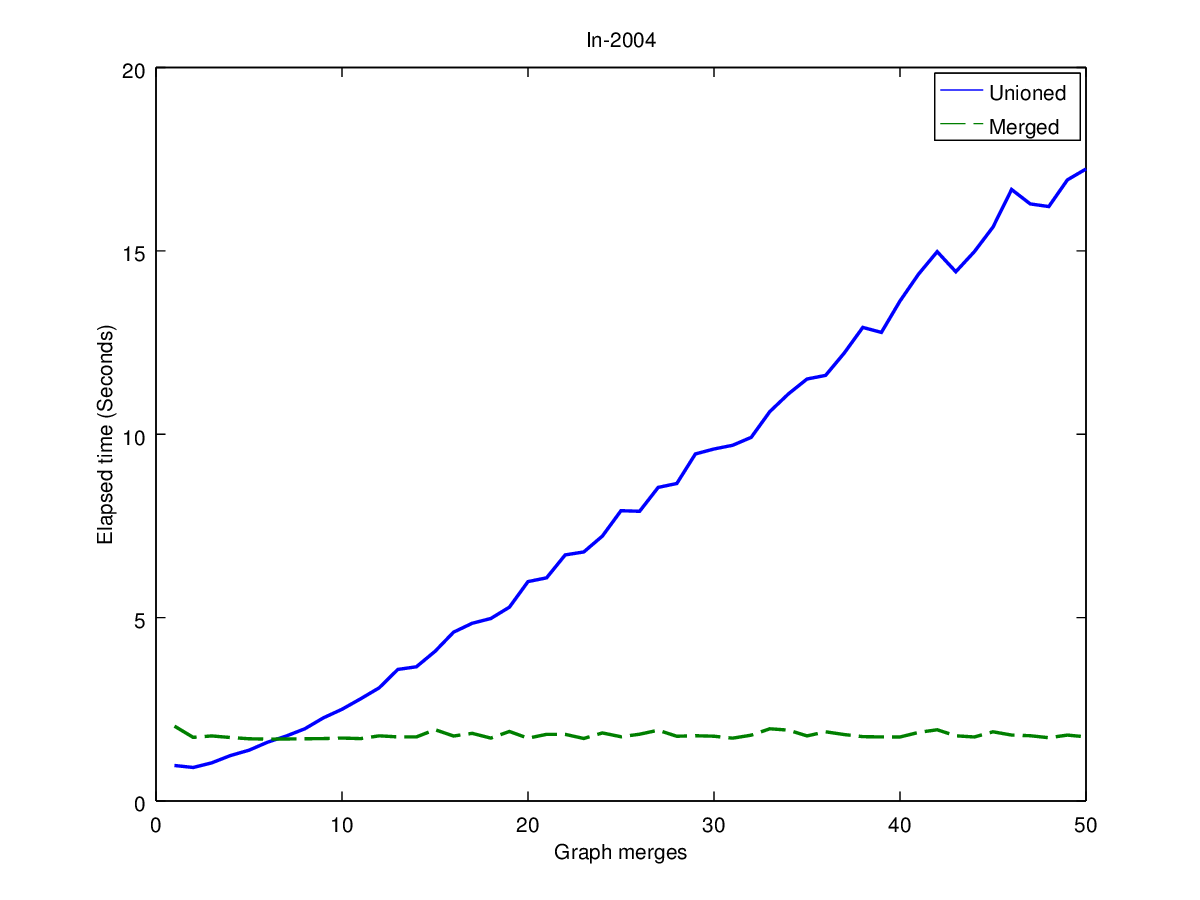
\includegraphics[width=14cm]{firstIterationUnionVsStored}    
\captionsetup{justification=centering}
\caption {Benchmark of unioned versus directly merged graphs}
\label{fig:firstIterationUnionVsStored}
\end{figure}

\subsection{Merging two graph files}
A method to merge the raw format of two BVGraphs without the references has been developed. The merging speed improves \todo{Show and analyze Benchmark here} tenfold by ignoring the references and the space used by the graphs are approximately doubled. This merge method is more appropriate than the existing one as for the algorithm to be dynamic, modifications to the graph have to be done as quickly as possible. This method has two phases for each node. The first phase reads the intervals of both graphs and merge them. As the intervals in the graph files are sorted in ascending order by the start of the interval, this can be done in $O(n)$ time (see Appendix B). In the next step, the algorithm takes the smallest residual node from one of the graphs and writes it to the output graph. As the residuals are already sorted in ascending order in the graphs, only the current head residuals in the graphs need to be considered. If they are the same, it is written once and both file pointers are moved forward so that no duplicates are written. If the residual to be written is already included in one of the intervals, it is ignored. Using this developed method allows for merging very large graphs at a short amount of time.

\subsection{How we solved it}
Not yet completed

\section{HyperLogLog resize}
After new nodes have been added to the graph, new counters have to be created for them. The initial counters retreived by HyperBall are represented as an array of longs. We intend to keep this representation, as it has a very low amount of wasted memory usage. It also minimized the number of objects created on the heap. But as new counters are needed, the array must be resized. For this, a geometric expansion is used as it gives $O(1)$ amortized time per insertion \cite{dynamicarrays}. In the geometric expansion the array capacity is increased by a factor. This is how the standard implementation of ArrayList in Java is dynamically increased. A larger factor implies an on average small number of copies per inserted elements but a high amount of unused space. The amortized number of copies per inserted element for a factor $r$ is roughly $\frac{1}{(r-1)}$ and the average unused space is $\log(r)*\frac{r}{(r-1)} - 1$. \cite{dynamicarrays}

Under the assumption that the graph expands slowly relative to its size, resizing events will be sparse and a large factor would mainly imply a large amount of unused memory. Therefore, it is more beneficial to let the array increase by a small factor. With the factor $r = 1.1$, an average of $4.8$\% space is unused and every element will on average be copied $10$ times.

\section{Updating counters}

After an edge has been added to the graph, the next step is to update the counters of all nodes affected by the insertion. Let $e = (u,v)$ be an edge added to the graph. All the nodes reachable from $v$ have to be propagated to the nodes that can now reach $v$ via $u$. Propagation means that all newly reachable nodes are hashed and inserted into the counters of the nodes that now reach them. This is performed in two phases, the collecting-bfs and the propagating-bfs.

The collecting-bfs is responsible for retrieving which nodes $v$ can reach. The collecting-bfs performs a bfs in the graph from $v$. For every level $i$ in the bfs, all nodes in the current frontier in the bfs are added into a HyperLogLog counter. This counter represents all nodes that $v$ reached in $i$ steps. The collecting-bfs completes at level $h-1$ and returns a $h$ long list of counters. The $h$'th step is not needed as only $v$ itself can reach this level.

The propagation-bfs is responsible for updating the counters of all nodes that now reach $v$, as they might have changed by the insertion. To find all nodes that can reach $v$, a bfs is performed from $u$ in the transpose of the graph. For every level $i$ in the bfs, the frontier of nodes in the bfs can reach all nodes that the collecting-bfs reached in $h-1-i$ steps. To update the counters of the nodes at level $i$, the current counters of the nodes are merged with the $h-1-i$ counter retrieved in the collecting-bfs. The propagation-bfs stops after $h-1$ steps after which all affected node counters have been updated.

\todo{Insert proof of correctness here}

\subsection{Optimized Breadth-first search}

A problem with the two phase algorithm described above is that it only supports single insertions at a time. Instead of adding each edge separately, they can be bulked into a set of edges to add. By bulking the edges several BFS's can be performed at the same time. The algorithm MS-BFS \cite{msbfs} does several BFS's at the same time very effectively and will be used in the algorithm. \todo{Show benchmark between std bfs and ms-bfs}

As the BFS can be pruned after traversing $h-1$ steps, there needs to be a way to stop the individual BFS's at that point. This was solved by implementing a method to pass the MS-BFS a visitor function (not related to the common Visitor design pattern). The visitor will be called every time a group of BFS's have reached a node. The group of BFS's that reached the node is represented as a list of bits and is passed to the visitor. If the visitor wants to stop the propagation of a BFS from this node it can clear the corresponding bit. No modifications to the algorithm needs to be done as MS-BFS already use a list of bits to propagate the BFS's.

Additionally, it is desirable to send data along with the BFS's. For this, a new concept called Travelers is introduced. The purpose of the traveler is to bring initial data from the BFS's and merge the data if several BFS's reach a node at the same time. This may prevent calculations that would otherwise need to be done in all or many of the visitors by removing the need to loop through which source nodes that reached the node. Travelers have to be able to merge to not increase the space complexity of the algorithm. The travelers are then passed to the visitors so they can use the data provided by the travelers. 

\section{Node history}

MS-BFS speeds up the algorithm significantly, but further optimizations can be done to the individual BFS's. To update a counter, the algorithm has to do two BFS's for every edge added. A large portion of the time spent by the algorithm will be doing these BFS's. Therefore, the ability to prune BFS's early would imply a large time improvement of the run time. Currently, the collecting-bfs must traverse the graph $h$ steps to gather all data needed. This is because every node only keeps track of its registers resulted by a search in $h$ steps. But if all nodes also keeps track of its registers in $h-1$ steps, then the collecting-BFS would only need to traverse $h-1$ steps as in the $h-1$'th step it could use the $h-1$ history of all nodes to calculate the $h$'th step. For every extra history level added, the collecting-BFS can stop one step earlier. So by saving every history level of all nodes, the collecting-BFS only needs to visit the immediate neighbors of a new node $v$ to be able to calculate the counter of $v$. 

During the HyperBall phase of the algorithm, the intermediate counters in HyperBall can be used to calculate all history levels of all nodes. HyperBall works in iterations, synchronizing all nodes between every iteration. During the $i$'th synchronization, the counters will represent the $i$'th level of all nodes history. So instead of only using the last level from HyperBall, all levels are saved. The $h'th$ level will be referred to as the top counter and level $0$ to $(h-1)$ as history counters. All levels combined will be referred as counter collection.  

Every node now has a list of its history which has to be updated with every edge update. For an edge $e = (u,v)$ inserted, the collecting-BFS has to gather the node history from all neighbors of $v$ and merge them into one. The merged history together with the $v$ itself added to them becomes $v$'s own history and counter. Then the propagation-BFS has to propagate this history in the transpose of the graph. These merging operations can be performed during the current BFS's and does not affect the time complexity of the bfs's.

With node history the algorithm has $O(hn \log \log n)$ space complexity as the top counter uses $O(n \log \log n)$ and the history counters use $O((h-1)n \log \log n)$. To insert an edge $e = (u,v)$, the two previous BFS's used $O(m)$ operations per BFS but with node history the collection-BFS use $O(\Delta_v)$ operations, where $\Delta_v$ is the out degree of node $v$. The time complexity of the node history version is then $O(m + \Delta_v)$. In practice, this means a large improvement as it often holds that $\Delta_v << m$.

Node history speeds up the algorithm but also uses extra space that, for large graphs, can be quite extensive. To create an algorithm that balances the gained speed versus the extra memory usage, the history could be saved for only a subset of nodes. These nodes should be picked so that as few nodes as possible need to save their history while keeping the BFS distance as short as possible. The algorithm to determine these nodes have to be very fast to avoid affecting the running time of the algorithm. It would also have to be dynamic to be able to continuously determine which nodes that should be included in the set.

\subsection{Vertex cover}
One way to determine which nodes that should keep their history is to use the nodes that are in a minimum vertex cover $VC$. Only saving the node history on nodes that are part of the $VC$ can significantly improve space usage, yet the BFS can still be bounded. The trick here is that for all nodes $u$, it holds that $u \in VC \vee \forall e = (u,v) : v \in VC$. Then, when the collecting-BFS searches from a node $v$ it will take at most two steps until it reach a frontier of only nodes in the vertex cover. From this frontier, the collecting-BFS can calculate $v$'s history and counter by merging the frontiers collection histories. The collection-BFS is now bounded by two steps, resulting in $O(\Delta_v + \sum_{u \in \delta^+_v}{\Delta_u}) $ operations. The top counter uses the same space but the history counters now use $O((h-1)|VC| \log \log n)$, so the total space complexity for the counter collection is $O(((h-1)|VC| + 1 )\log \log n)$.

\subsubsection{Dynamic minimum vertex cover}
There is a requirement to, at all times, keep track of which nodes are in the vertex cover. This requires a fully dynamic minimum vertex cover algorithm. However, as minimum vertex cover is NP-complete, approximation algorithms must be used. The choice of fully dynamic approximate minimum vertex cover algorithm depends on the ratio between the number of insertions and deletions. A simple greedy algorithm can maintain a $2$-approximation in $O(1)$ time per insertion and $O(n)$ time per deletion \cite{2appdynvc}, while an algorithm that partition the nodes can maintain the same approximation in $O(\log(n))$ amortized time per insertion and deletion \cite{2appdynvclogn}. In our case, deletions will be very sparse in the data stream, which is why the greedy algorithm was chosen. The greedy algorithm also have the property that if a deleted edge was not part of the maximal matching previously, it deletes the edge in $O(1)$ operations. For dense graphs, only a small amount of the edges will be in the maximal matching, which makes it in many cases perform very quickly in deletions as well. 
 
\subsubsection{Directed graphs}
As the standard minimum vertex cover problem is defined for undirected graphs the problem have to be slightly modified. The new problem description is as follows; given a directed graph $G = (V,E)$, we wish to select a minimum cardinality subset $V' \subseteq V$ such that $\forall e = (u,v) \in E, u \in V' \vee v \in V'$. The problem is still NP-complete as undirected graphs are a special case of directed graphs. 

By the same reasoning as in the undirected case, a maximal matching is a $2$-approximation of the generalized problem. However, the greedy algorithm needs to be modified to support directed edges. The only case affected is when an edge in the maximal matching is deleted. Previously, the algorithm scanned the endpoints of the deleted edge for uncovered edges. With directed edges, both incoming and outgoing edges must be verified. This can be solved by saving both directions into each node, as in the undirected case. However, this would imply a doubling in space usage for the graph. Also, as deletions are expected to be rare, saving both types would in most cases be unnecessary. Instead, the problem can be solved by a complete edge scan. An edge scan can detect all edges, incoming and outgoing, that are possibly affected. This requires no extra information added, but implies a larger time complexity for deletions. Instead of $O(n)$ operations, deleting edges now take $O(m)$ operation per deletion. Fortunately, the amortized number of edge scans required per deletion can be reduced by performing deletions in bulk. A single edge scan is sufficient for detecting all the affected edges of any sized bulk of deletions. 

\subsubsection{Benchmark insertions}
The selected greedy algorithm was benchmarked with the publicly available it-2004 graph. It-2004 contains 41.291.594 nodes and 1.150.725.436 edges. Starting with an empty graph, every edge was sequentially inserted from it-2004 into the dynamic vertex cover. Both the time and heap size was measured over the number of inserted edges, see figure \ref{fig:firstIterationDvc}. This shows roughly 29.5 million inserted edges per second. The memory used mainly depends on the number of nodes. The heap size increased from 0.93GB to 1.51GB, hence 0.58GB memory was used to remember the vertex cover. 0.58GB equals 622770258 bytes, making it an on average 15 bytes per node. 

% 15 bytes per node is nice. Should be 8 + 8 bytes + 1 bit p = 16.125 bytes so seems perfect!

\begin{figure}[h]
\centering
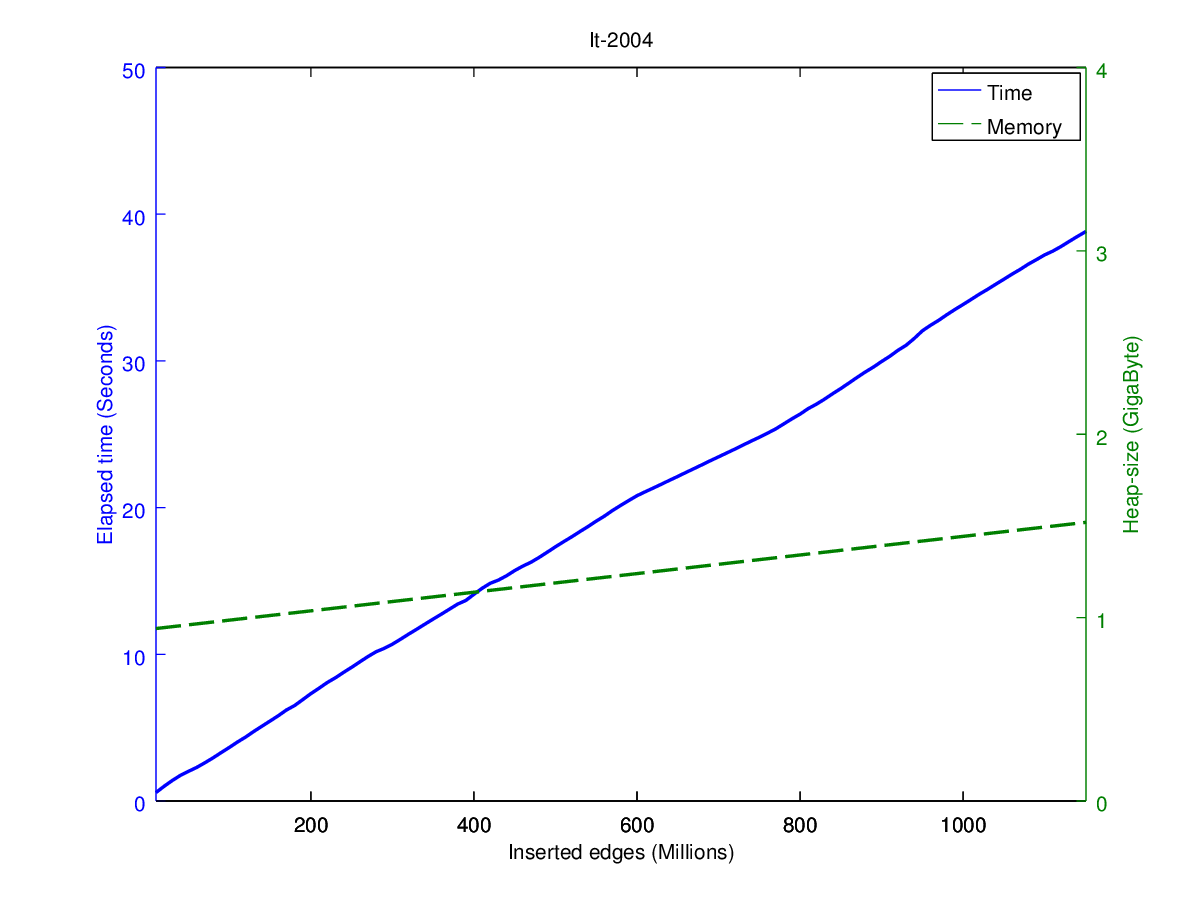
\includegraphics[width=12cm]{firstIterationDvc}    
\captionsetup{justification=centering}
\caption {Benchmark of sequential insertions in 2-approximative dynamic vertex cover}
\label{fig:firstIterationDvc}
\end{figure}

\subsubsection{Benchmark deletions}
To test the performance of sequentially deleting edges the publicly available in-2004 graph was used. In-2004 contains 1.382.908 nodes and 16.917.053 edges. The test was performed by first inserting all edges into the dynamic vertex cover and then taking the first 2.000 edges in the graph file and sequentially delete them, see figure \ref{fig:firstIterationDvcDeletion}. The benchmark shows that for this relatively small graph the algorithm achieves roughly 25 deletions per second. As this speed will decrease linearly with the number of edges in the graph, edges must be deleted in bulk.

\todo{Implement bulk deletions and compare with sequential}

\begin{figure}[h]
\centering
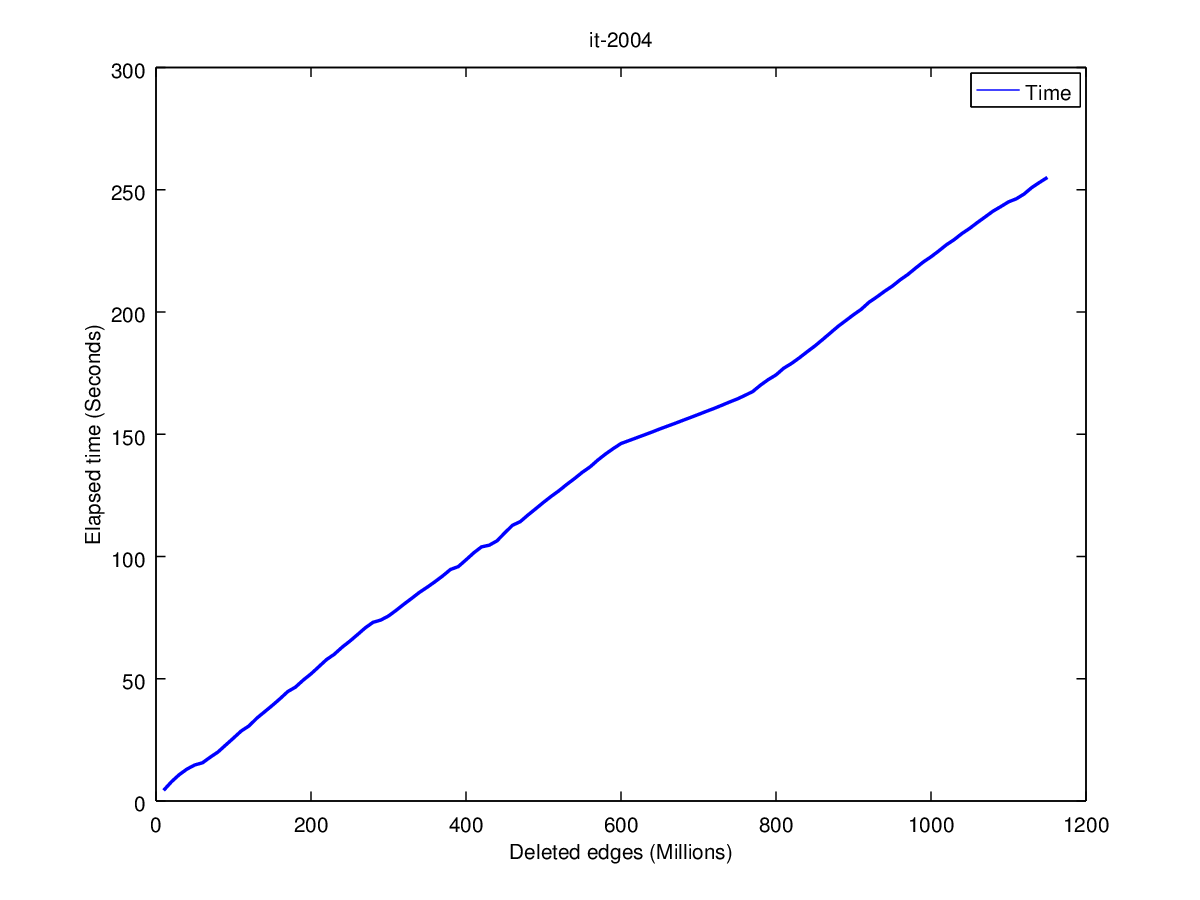
\includegraphics[width=12cm]{firstIterationDvcDeletions}    
\captionsetup{justification=centering}
\caption {Benchmark of sequential deletions in 2-approximative dynamic vertex cover}
\label{fig:firstIterationDvcDeletion}
\end{figure}

\subsection{Edge insertion}

Edge insertion now is divided into four steps. The first step is checking if the edge contains any new nodes. New nodes are added to the graph and the top counter is, if necessary, resized to fit new counters of the new nodes. The second step is to check if any new node needs to be added into the vertex cover. For all new nodes in the vertex cover, memory is allocated in the history counters. The third step is calculating the history of the nodes added to the vertex cover. Lastly, the new history is propagated with a BFS in the transpose of the graph to update the counters of nodes affected by the insertion. After these four steps all nodes will have an approximate neighborhood function in their top counters and all nodes in the vertex cover will have their history counters updated. 

\subsubsection{History propagation}

When a new edge $e = (u,v)$ is added to the graph, many nodes that has a path to $u$ will contain outdated information. The algorithm works by propagating the history of $v$ through the transpose of the graph. If $v$ is not in the Vertex Cover, the history needs to be calculated from the neighbor nodes. The algorithm is presented in pseudo code, see figure \ref{fig:history_propagation_algorithm}.

\begin{figure}[h]
    \begin{lstlisting}[mathescape]
e = (u,v) //Edge to add
if(isInVertexCover(v))
    H$_v$ = H(v);
else
    H$_v$ = union of the history of the neighbor nodes;
In BFS; source: u, current node: z, at depth: d{
    d = d+1;  // We perform a BFS from u so the actual depth 
              // (from v) is one higher
    if(isInVertexCover(z)){
        foreach 0 $\leq$ i $<$ h+1-d{
            H(z,i+d).union(H$_v$(i));
        }
    }else{
        H(z,h).union(H$_v$(h-d));
    }
}
    \end{lstlisting}
    \caption{History propagation}
    \label{fig:history_propagation_algorithm}
\end{figure}

To speed up the algorithm, it needs to be modifier to handle several edges at once. In this case the traveler support of the MS-BFS algorithm can be used. This means that the data provided by the traveler can be used instead of looping through all the source nodes. The travelers will contain the counter registers of their respective source node. When the travelers merge they can take the union of their registers. They also only need to keep the $h+1-depth$ top-most counters as the others won't reach further anyway. In the visitor the data from the traveler is joined with the existing counters of the visited nodes. The merge function for the traveler is constructed as in figure \ref{fig:history_propagation_traveler}.

\begin{figure}[h]
    \begin{lstlisting}[mathescape]
Input: t1,t2 = travelers to merge (HyperLogLog counters)
       d = depth of the BFS
Output: a new traveler
tOut = t1.clone
foreach 0 $\leq$ i $<$ h+1-d{
    tOut$_i$ = tOut$_i \cup $t2$_i$
}
return tOut
    \end{lstlisting}
    \caption{History propagation traveler}
    \label{fig:history_propagation_traveler}
\end{figure}

The visitors only have to be slightly modified to make us of this traveler. The only difference is that the visitor use the counter history from the traveler data instead of taking it from the source nodes.\\\\
\textit{Theorem: } After an update all nodes have had all reachable nodes added to their counters \\\\
\textit{Proof: } This will be shown by an inductive proof. 

\begin{addmargin}[2em]{0em}
\textbf{Base case: } The history of the nodes are initially correct as the initial state is produced by HyperANF which is proven to be correct. \\\\
\textbf{Induction hypothesis: } The counters are correct after $p$ updates.\\
\textbf{Induction case: } Take any two nodes $u,v$ where $u$ reach $v$ in at most h steps. In the $p+1$ update there are two cases. \\

\textbf{$u$ reached $v$ in update $p$}) By the induction hypothesis it holds that the counters where correct in update $p$, hence $v$ have been added to the counter of $u$.\\

\textbf{$u$ did not reach $v$ in update $p$}) As $u$ reach $v$ in update $p+1$, there must be a path $P$ from $u$ to $v$ where an edge has been added. Let $e = (a,b) \in P$ be the new edge of maximum hops from $u$. As $u$ reach $v$ in at most $h$ steps it holds that $|P| \leq h$.
 As there are no more new edges between $b$ and $v$, combined with the induction hypothesis the counter of $b$ was correct in the update $p$ and included $v$. By the algorithm, the propagation step will traverse $h$ steps from $b$ and as 
$|P_{u \rightarrow b}| \leq |P| \leq h$ the propagation from $b$ will have reached $u$ and added $v$ to its counter. $\blacksquare$


\end{addmargin}

\section{Deletions}

\section{Graph construction}

